\documentclass[spanish,a4paper,11pt]{article}

\usepackage{latexsym,amsfonts,amssymb,amstext,amsthm,float,amsmath}
\usepackage[spanish]{babel}
\usepackage[utf8]{inputenc}
\usepackage[dvips]{epsfig}
\usepackage{doc}
\usepackage{graphicx}

\begin{document}
\title{Aproximación del número $\pi$}
\author{Anabel Estévez Carrillo \\ Práctica \#10}
\date{11 de abril de 2014}

\maketitle

\begin{abstract}
El objetivo de este informe es exponer un programa escrito en el lenguaje de programación Python en el que se aproxime 
el valor de $\pi$. Además, se tratara de profundizar en los conocimientos adquiridos sobre \LaTeX{}, realizando un informe.
\end{abstract}

%+++++++++++++++++++++ Comenzamos con la primera sección +++++++++++++++++++++++++++++

\section{El número pi y su historia}

El número pi, representado por la letra griega $\pi$, equivale a la constante que relaciona el perímetro o longitud de una 
circunferencia con su diámetro. Es un número irracional y una de las constantes matemáticas más importantes.

Se estima que ya en el año 2.000 a.C. los babilonios tuvieron un acercamiento al averiguar que la circunferencia de un 
círculo suele ser poco más de tres veces el equivalente a su diámetro. Sin embargo, no fue hasta el año 225 a.C. cuando 
Arquímedes de Siracusa inició su teoría matemática. La misma se fue perfeccionando a lo largo de los siglos y en 
1706 el matemático William Jones usó por primera vez su símbolo $\pi$, aunque fue Leonhard Euler el que lo popularizó
 a partir de 1737. 

%+++++++++++++++++++++ Comenzamos con la segunda sección +++++++++++++++++++++++++++++

\section{Aproximaciones de $\pi$}

El valor de $\pi$ se ha obtenido con diversas aproximaciones a lo largo de la historia. La búsqueda del mayor número de 
decimales del número $\pi$ ha supuesto un esfuerzo constante de numerosos científicos a lo largo de la historia.
Una forma exacta de poder calcular $\pi$ es la fórmula de Machin, descubierta en 1706. De este modo, 
$\pi$ se puede calcular mediante integración:

$$\int_{0}^{1} \!\frac{4}{1+x^2}\, dx = 4(atan(1) -atan(0)) = \pi $$

Esta integral\footnote{La integral debe estar definida entre 0 y 1.} se puede aproximar numéricamente con una fórmula de cuadratura.

%+++++ Primera subsección de la sección dos ++++++

\subsection{Regla del punto medio}

Si se utiliza la regla del punto medio se obtiene:

\begin{center}
$ \pi \approx \frac{1}{n} \sum\limits_{i=1}^{n}f(x_i)\,$,
con $f(x) = \frac{4}{(1+x^2)}\,$,
$x_i = \frac{i - \frac{1}{2}}{n}$,
para $i = 1, \dots, n$.
\end{center}

%+++++++++++++++++++++ Comenzamos con la tercera sección +++++++++++++++++++++++++++++

\section{Calculando $\pi$ con python}

Vamos a escribir un programa\footnote{Puede ver el código propuesto accediendo al repositorio llamado prct06 en github} que utilize la regla del punto medio expuesta anteriormente para calcular una aproximación de $\pi$. El recibirá
como entrada el número de subintervalos con los que se desea abordar la aproximación del número $\pi$.\\
\cite{python}
A partir de este valor, se deben calcular y mostrar por la consola:

\begin{enumerate}
  \item
    Los extremos de los subintervalos.
  \item
    El punto $x_i$.
  \item
    El valor de de la función de aproximación de $pi$, $f(x_i)$.
  \item
    El resultado de la aproximación.
  \item
    La constante $pi$ con treinta y cinco decimales.
\end{enumerate}

%+++++ Primera subsección de la sección tres ++++++

\subsection{Ejemplo}
Por ejemplo, si se utilizan 4 subintervalos, la salida debería ser: 
\begin{footnotesize}
\begin{verbatim}
Introduzca el número de intervalos (n > 0): 4
Subintervalo: [0 , 0.25] x_i: 0.125 fx_i: 3.93846
Subintervalo: [0.25, 0.5 ] x_i: 0.375 fx_i: 3.50685
Subintervalo: [0.5 , 0.75] x_i: 0.625 fx_i: 2.8764
Subintervalo: [0.75, 1 ] x_i: 0.875 fx_i: 2.26549

El valor aproximado de PI es: 3.14680051839
\end{verbatim}
\end{footnotesize}
En forma de tabla:\\
\cite{latex}
\begin{table}[!h]
\label{Mitabla}
\begin{tabular}{lrcc}
Subintervalo & xi & fxi\\
\hline
0 & 0.25 & 0.125 & 3.93846\\
0.25 & 0.5  & 0.375 & 3.50685\\
0.5 & 0.75 & 0.625 & 2.8764\\
0.75 & 1  & 0.875 & 2.26549\\
\end{tabular}
\end{table}

En la tabla \ref{Mitabla} aparece el ejemplo anterior.

%+++++++++++++++++++++ Añadimos una imagen +++++++++++++++++++++++++++++

\section{Imagen}
\begin{figure}[h]
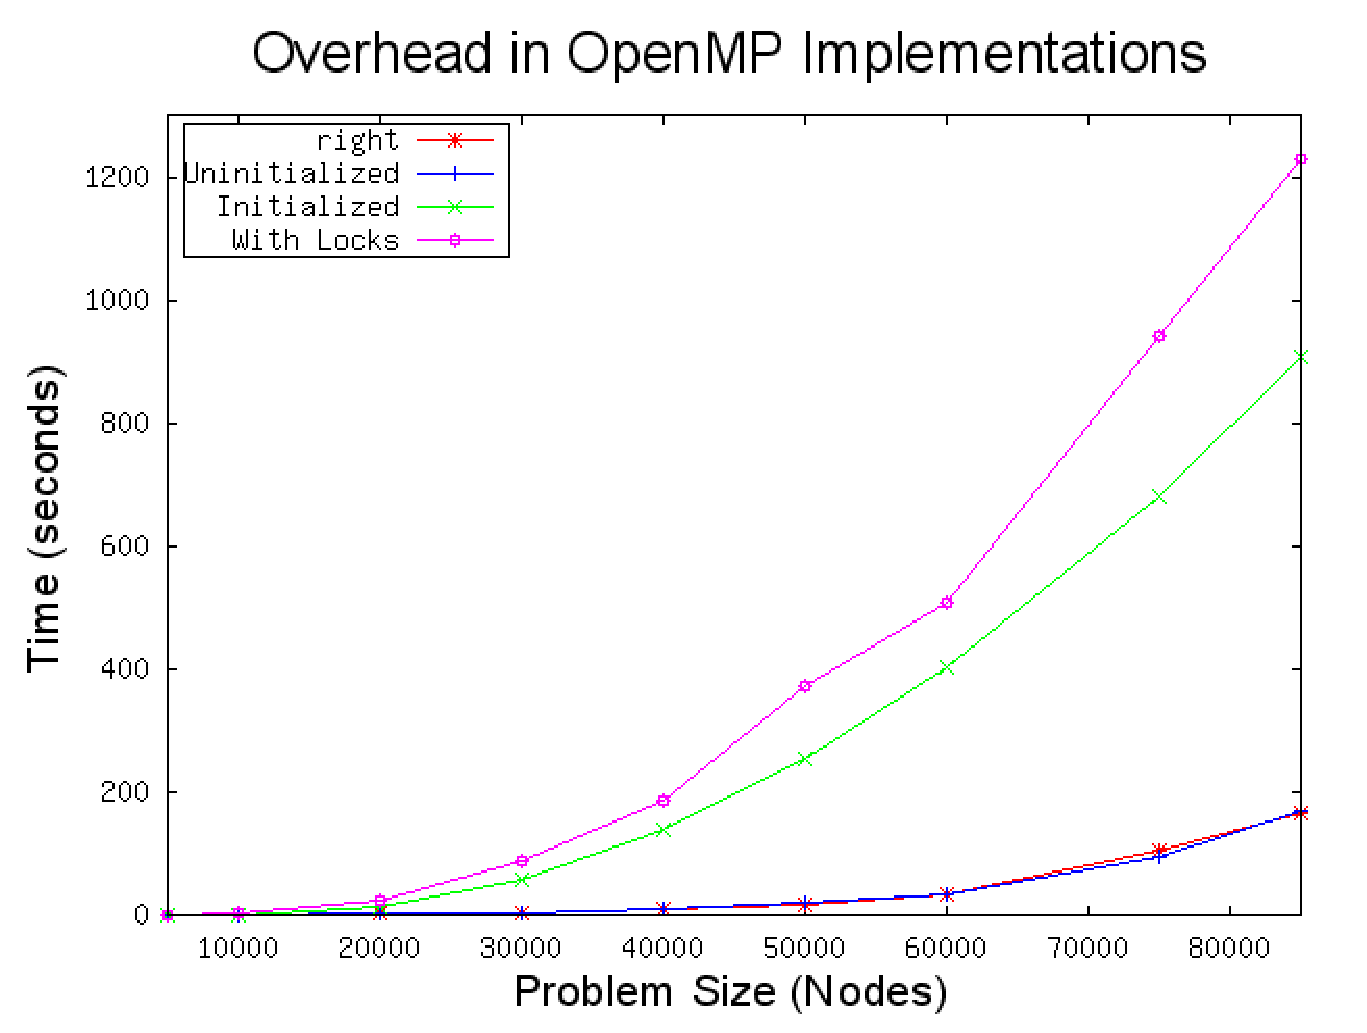
\includegraphics[scale=0.5]{figura1.eps}
\caption{Imagen eps}
\label{Mifigura}
\end{figure}

En la figura \ref{Mifigura} aparece un gráfico que representa datos estadísticos.

\end{document}


%+++++++++++++++++++++ Comenzamos con la bibliografia+++++++++++++++++++++++++++++

\begin{thebibliography}{2}
\bibitem{python} Tutorial de Python. http://docs.python.org/2/tutorial/
\bibitem{latex} Tutorial de Latex. http://latexlive.files.wordpress.com/2009/04/tablas.pdf
\end{thebibliography}
